% !TEX root = Sotsuron_main_v3.tex
%%Chap2
本章では,本研究で取り扱うCTS問題 (Continuous similarity search for Text Streams) 問題\cite{kubo}の定義を述べる.

\section{CTS問題}

CTS問題ではユーザ$A$を$A$が投稿したテキストの集合で特徴づける.テキストは単語の
集合である.例えば,Twitterのユーザを投稿したtweetで特徴づけるということになる.
各ユーザ$A$が単位時間毎に新しいテキストを1つ投稿するストリーム環境を想定する.

各データストリーム$A$には幅$W$のスライディングウィンドウが設定され,スライディングウィンドウは$A$に到着した直近$W$個の要素が含まれる.
つまり,CTS問題では時刻$T$のユーザ$A$が保有するテキスト集合$A_T$は,$A_T=\{a_{T-W+1},a_{T-W+2},...,a_T\}$となる.時刻$T$か
ら$T+1$に更新された時,図\ref{sw}のようにスライディングウィンドウに$a_{T+1}$が到着し,$a_{T-W+1}$が離脱する.
\begin{figure}[htb]
  \begin{center}
    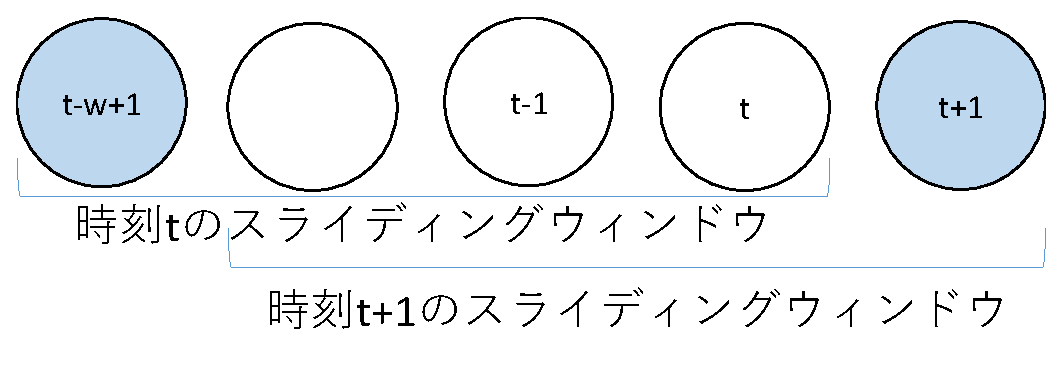
\includegraphics[clip,width=\linewidth]{img/sw.eps}
    \caption{スライディングウィンドウモデル}
    \label{sw}
  \end{center}
\end{figure}

CTS問題は,多数のユーザのテキストストリームを保持したデータベース$D$とクエリユーザ$V$のテキストストリームが与えられて,
毎時刻クエリ$V$とのユーザ間類似度$\mbox{sim}(V_T,U_T)$が閾値$\epsilon_u$以上であるすべてのユーザ$U$を$D$から検索する
継続的なレンジ探索である.したがって,スライディングウィンドウが変化する度に類似度判定結果を更新することが要求される.

ここでテキスト集合$V_T,U_T$間の類似度 $\mbox{sim}(V_T,U_T)$は以下のように定義される.
\begin{enumerate}
\item $V_T$と$U_T$の類似テキストペア間に辺を張り2部グラフ$G(V_T,U_T)$を構成する.
ここで2つのテキスト$o\in V_T,o'\in U_T$が類似テキストペアとなる条件は,$o,o'$を単語集合と見なした時に
そのJaccard類似度
\begin{align}
\label{match}
\tau (o,o')=\frac{|o\cap o'|}{|o\cup o'|}
\end{align}
が$\tau (o,o')\geq \mbox{閾値}\epsilon_{doc}$という条件を満たすことである.直感的には,
共通単語を多く保有するテキストペアが類似テキストペアとなる.閾値$\epsilon_{doc}$はレンジ探索の際に指定されるパラメータとなる.
\item グラフ$G$の最大マッチング$M$のサイズ$|M|$を$\mbox{sim}(V_T,U_T)$とする.
\end{enumerate}

なお,上記で説明した問題は単位時間毎にテキストが投稿されるとしているが,本稿で扱うすべてのアルゴリズムは数単位時間ごとにテキストが投稿されるような,ユーザごとに一定でない時間間隔でテキストが投稿される場合にも対応可能である.

\section{近似レンジ探索}\label{kinjirange}
CTS問題は毎時刻スライディングウィンドウの内容が変化するため,クエリユーザ$V$とデータベース上のすべてのユーザ$U$との類似判定結果を毎時刻更新する必要がある.よって,最大マッチングを毎時刻求める必要がある.
しかし,データベース上の全ユーザに対して存在する二部グラフの最大マッチングを毎時刻求めることは計算量が大きくなってしまい困難である.そこで久保ら\cite{kubo}の研究でああるように本研究でも類似の定義をユーザ間の最大マッチングサイズが閾値$\epsilon_u$を超えるのではなく,ユーザ間の極大マッチングサイズが閾値$\epsilon_u$を超えるかとして扱う.
類似度に極大マッチングサイズを用いれば,一度マッチングが成立したテキストペア$(o,o')$はそのどちらかがスライディングウィンドウから離脱するまでマッチングを維持でき,マッチング判定の処理を省略することができるので,類似度の算出に必要な計算量が小さくなると考えられる.


\section{ユーザ間類似度}
以上より本問題は極大マッチングサイズをもとにユーザ間類似度を決定しているが,Zhangら\cite{zhang2021clustering}は異なる基準を用いてユーザ間類似度を定義している.
Zhangらの研究では,CTS問題と同様にJaccard類似度が閾値以上になるテキストペアに辺を張り二部グラフを構築しているが,極大マッチングサイズではなく,二部グラフの最大重みマッチングサイズをユーザ間類似度としている.つまりCTS問題ではJaccard類似度が閾値$\epsilon_{doc}$となるテキストペアをすべて同じ価値としてみなしているが,Zhangらの研究ではJaccard類似度を重みととらえ,テキストペア自体に価値を設定している.最大重みマッチングを用いることでより正確にユーザ間類似度を測ることができると考える.

しかし,\ref{kinjirange}節であるように最大マッチングを求めることは計算量的に困難である.これが最大重みマッチングの場合,さらに計算量が大きくなることが予想される.よって計算量の観点から本問題のユーザ間類似度に極大マッチングサイズを用いることは妥当だと考える.

---

スライディングウィンドウ



Minhash

集合間で類似度を検索する方法の一つとして,Min-hashがある.Min-hashは,集合に対する確率的なハッシュ関数であり,Jaccard係数を用いた集合間類似検索を高速化するための技術である.Min-hashは計算されたハッシュ値が一致する確率はJaccard係数と一致するという性質を持つ.類似集合ほどハッシュ値が一致しやすいという性質を持つ.


Minlist

多重集合に対するハッシュ値更新アルゴリズム

3. 問題点

3.1. Minlistの探索回数の増大

そもそもなぜMinlistの探索が必要なのか?

Minlistは,探索回数が多い.多重度のヒストグラムは要素Nが到着したときの到着時刻tをすべて記録している.しかしこの実装だとヒストグラムの要素数はスライディングウィンドウのサイズになる.このヒストグラムの到着時刻は.割り当て値であるハッシュ値の更新に使用する.要素γがウィンドウ内に存在する間、γ,et+1 間にラベルがl(et+1)となる要素がn個ある。よって、要素γ の存在尾期間中のet+1の割り当て値はπ(l(et+1)n) より大きくならなない。よってであれば,要素γ をMinlist から削除してよい.最後にMinlist の一番後ろにet+1 を挿入し,π(et+1) がMinlistの最小値を更新するかをチェックする.現在のハッシュ値よりπ(et+1) が小さいならば,ハッシュ値を更新する.

3.2. 割り当て表のメモリ割り当てのメモリが大きい

Min-hashを割り当てるためのハッシュ値の割り当て表のサイズは要素の種類数×多重度になる.しかし割り当て値の修正を行っているため,多重度が大きくなればなるほど割り当て値の変動する確率が下がる.そのため割り当て表はサイズが大きくなればなるほど意味を持たない割り当て値を多く持つことになりメモリ使用量に無駄が生じる.

3.3. ヒストグラムのメモリ割り当てのメモリが大きい

ヒストグラムのサイズは,要素の種類数の数だけ配列のサイズを確保する必要がある.ストリームデータが複数個になると,その数だけヒストグラムのメモリを確保する必要がある.また,スライディングウィンドウのサイズに対して要素の種類数が多いとヒストグラムの要素が0である比率が大きくなる.実質的に意味を持たない要素が多くなる.

4. 提案手法

3.1. Minlistの探索にSerch Limitを設ける



3.2. Active Indexを用いた割り当て表の作成

3.3. Count-Min Sketchを用いた多重度の近似ヒストグラムの作成